% ACM acmart v2.20 (2026-08-16), vendored unmodified alongside this file.
% Compile from this directory: pdflatex milestone; bibtex milestone;
% pdflatex milestone; pdflatex milestone. See README.md for the local build script.
\documentclass[sigconf,nonacm]{acmart}
\usepackage{amsmath}
\usepackage{listings}
\settopmatter{printacmref=false,printfolios=true}
\setcopyright{none}
\renewcommand\footnotetextcopyrightpermission[1]{}
\acmDOI{}
\acmISBN{}
\acmConference[CS 5787 Milestone]{CS 5787: Deep Learning -- Project Milestone}{November 2026}{Cornell University}
\acmYear{2026}
\title{Training-Free Block Reuse in Diffusion Transformers}
\subtitle{Project Milestone: Removal, Residual Damping, and Attention Projection}
% Replace these TODOs before submission; duplicate the author block for each student.
\author{TODO: Student name(s)}
\authornote{Cornell NetID(s): \texttt{TODO}.}
\affiliation{\institution{Cornell University}\city{Ithaca}\state{New York}\country{USA}}
\email{TODO@cornell.edu}
\renewcommand{\shortauthors}{TODO: Student name(s)}

\begin{abstract}
We investigate whether a frozen diffusion transformer can use fewer distinct
blocks while preserving its generated outputs. Using pretrained DiT-XL/2, we
compare block removal, reuse of the preceding retained block, damped reuse,
and reuse with Exclusive Self-Attention (XSA). A completed pilot generates
20 class--seed-matched images per method on ten Imagenette classes. Removing
two of 28 blocks reduces unique DiT parameters by 7.08\% and mean measured
latency from 7.642 to 6.932 seconds per image. Damped reuse yields lower
mean paired LPIPS than unscaled reuse (0.547 versus 0.614), while retaining
28 block calls. These are descriptive pilot observations: the available
FID estimates use only 20 generated images and do not establish a quality
ranking. We formalize the methods, document the evaluation protocol, and
identify the held-out and multi-reuse experiments needed for the final report.
\end{abstract}
\keywords{diffusion transformers, training-free compression, block reuse, perceptual evaluation}
\begin{document}
\maketitle

\section{Problem and Research Basis}
Diffusion Transformers (DiTs) perform many expensive denoising passes through
a stack of distinct transformer blocks~\cite{peebles2023dit}. We ask:
\emph{Can selected blocks be replaced by retained weights without retraining,
and can residual damping or attention projection reduce the resulting output
shift?} The goal is to understand the trade-off among unique parameters,
execution cost, and image preservation; sharing weights alone need not reduce
the number of executed blocks.

Our proposal draws on six papers. Chen et al.~\cite{chen2026trainingfree}
retrofit recurrence into frozen language models and motivate controlled
residual updates. Peebles and Xie~\cite{peebles2023dit} provide our model and
sampling baseline. TeaCache~\cite{liu2025teacache} reuses outputs across
denoising timesteps; our intervention instead reuses \emph{weights across
depth slots} within a timestep and computes fresh activations. ELT's
intra-loop self-distillation~\cite{goyal2026elt} and Looped-DiT's deep
supervision and self-modulating attention~\cite{chng2026loopeddit} train for
recurrence. We test a narrower, inference-only adaptation of XSA, without
their training losses. TPIPS~\cite{wang2026tpips} motivates aspect-conditioned
perceptual evaluation; its implementation is available as an optional metric,
but no TPIPS measurements are reported because it was disabled to limit
evaluation cost. Our pilot therefore does not reproduce the full methods or
benchmark claims of those papers.

\section{Formal Setting, Data, and Metrics}
Let $B_0,\ldots,B_{L-1}$ be the $L=28$ blocks of a frozen DiT, with hidden
state $h_s$ and conditioning $c_t$ at denoising timestep $t$. A common sampler
and VAE map a class--seed pair $(y_i,s_i)$ to an image $x_i^{(m)}$ for method
$m$; $m=0$ denotes the unmodified model. We compare candidates with fewer
unique parameters using the tuple
\begin{equation}
 \bigl(P_m/P_0,\ T_m/T_0,\ D_m,\ \widehat{\mathrm{FID}}_m\bigr),
 \qquad
 D_m=\frac1N\sum_{i=1}^{N}\mathrm{LPIPS}(x_i^{(0)},x_i^{(m)}).
 \label{eq:objective}
\end{equation}
Here $P_m$ counts unique DiT parameters, $T_m$ is mean synchronized latency,
and $D_m$ measures paired output deviation, not realism.

\paragraph{Data and preprocessing.}
We use Imagenette v2, a prepackaged ten-class ImageNet subset with 9,469
training and 3,925 validation images~\cite{howard2019imagenette}. The generation
labels are the \emph{original ImageNet IDs}
$\{0,217,482,491,497,566,569,571,574,701\}$, corresponding to tench,
English springer, cassette player, chain saw, church, French horn, garbage
truck, gas pump, golf ball, and parachute. They are stored in one class array;
Imagenette's local indices $0$--$9$ are not model class IDs.
The completed run uses two generated images per class per method
($N=20$; 100 images across five methods). A fixed real reference uses 500
images per class from Imagenette's \emph{training} split, selected without
replacement with reference seed zero. No model training is performed.
Real images are converted to RGB, resized with aspect-preserving bicubic
interpolation and center cropping to $256\times256$, then saved as PNGs.
Generated images are stored both as FP32 tensors in $[-1,1]$ and preview PNGs.

\paragraph{Perceptual and distributional evaluation.}
LPIPS uses the AlexNet v0.1 implementation on the saved tensors~\cite{zhang2018lpips}.
Clean-FID's clean Inception pipeline~\cite{parmar2022cleanfid} reads only
manifest-listed generated PNGs, excluding grids. FID compares the pooled
generated and real feature distributions~\cite{heusel2017fid}:
\begin{equation}
 \widehat{\mathrm{FID}}=
 \|\mu_g-\mu_r\|_2^2+
 \mathrm{tr}\!\left(\Sigma_g+\Sigma_r
 -2(\Sigma_g^{1/2}\Sigma_r\Sigma_g^{1/2})^{1/2}\right).
 \label{eq:fid}
\end{equation}
Both sets have equal class proportions. Comparing these ten-class outputs
against a 1,000-class reference would confound the intentional class
restriction with generation error. At $N=20$, the generated 2,048-dimensional
covariance has rank at most 19. Finite-sample FID is also model-dependently
biased~\cite{chong2020fid}; these scores are exploratory and cannot be compared
to published ImageNet FID-50K. All metrics and reference preparation run
after generation and are excluded from timing.

\section{Methods and Implementation}
All measured compressed methods remove the same fixed slots
$S=\{4,7\}$ (zero-based). Let $p(s)=\max\{j<s:j\notin S\}$ be the nearest
preceding retained source block and $R_j(h,c)=B_j(h,c)-h$ its residual.
At retained slots, every method applies $B_s$ normally. At a removed slot:
\begin{equation}
 h_{s+1}=\begin{cases}
 h_s,&\text{removal},\\
 B_{p(s)}(h_s,c_t),&\text{unscaled reuse},\\
 h_s+\alpha_s R_{p(s)}(h_s,c_t),&\text{damped reuse}.
 \end{cases}
 \label{eq:methods}
\end{equation}
Retained modules are registered once in a shared container. Thus removal has
26 block calls per forward pass; both reuse variants keep 28 calls but only
26 distinct blocks. Their source sequence begins
$0,1,2,3,3,5,6,6,8,\ldots,27$.

\paragraph{Damping: measured policy and current extension.}
The pilot uses fixed $\alpha_s=0.5$ \emph{only on replacement calls}. The
current implementation generalizes this to $\alpha_s=1/k_s$, where $k_s$
counts calls to that retained source, including its original call as $k=1$.
Successive extra calls use $1/2,1/3,1/4,\ldots$; counters restart for each
source and forward pass. With isolated removals $\{4,7\}$, both policies
have exactly the same scales. Consecutive removals are needed to test their
difference. This harmonic schedule is our adaptation, not Chen et al.'s
constant-$1/K$ substep scheme with anchoring~\cite{chen2026trainingfree}; we
do not claim the same numerical-integration guarantees.

\paragraph{XSA reuse.}
For a replacement call, compute fresh query, key, and value tensors using
the reused block. Given a token/head attention output $o$ and its current
self-value $v$, apply the parameter-free projection~\cite{chng2026loopeddit}
\begin{equation}
 \bar v=\frac{v}{\max(\|v\|_2,\epsilon)},\qquad
 o'=o-\langle o,\bar v\rangle\bar v,\quad\epsilon=10^{-8}.
 \label{eq:xsa}
\end{equation}
Our hooks filter the separate-head-equivalent tensor before post-attention
normalization and output projection, leaving DiT's conditioning, residual
gates, and MLP intact. Projection arithmetic is FP32; hooks are removed after
each call, including on failure. Ordinary retained calls remain unmodified.
This does not copy cached attention outputs or remove only the attention
matrix diagonal. We introduce no learned XSA parameters or deep-supervision
training.

\section{Completed Experiments and Preliminary Results}
\paragraph{Protocol.}
We use the official pretrained DiT-XL/2 $256\times256$ checkpoint and a shared
\texttt{sd-vae-ft-mse} VAE, 50 ancestral sampling steps, CFG scale 4.0, and
FP32. The completed comparison is the saved run
\texttt{team\_20261117T003651069722Z}. Its 20 validation pairs use seeds
10020--10039; initial noise is generated on CPU and the ancestral RNG is reset
for each matched pair. Calibration inputs are disjoint, but calibration-based
selection was not executed for this fixed-slot experiment. Measurements were
recorded on Apple Silicon/MPS under macOS 15.5 and PyTorch 2.15.0. MPS uses
deterministic-algorithm warnings, not a guarantee of bitwise reproducibility
across devices. Timing includes synchronized diffusion, VAE decoding, and CPU
transfer; it excludes loading, warmup, serialization, profiling, and metrics.

\begin{table}[t]
\caption{Completed ten-class pilot, $N=20$ per method. LPIPS is mean $\pm$
sample SD; latency is the measured mean in seconds. FID uses 5,000 real images
and has no estimated confidence interval. Smaller is better for these three
metrics. Differences are descriptive, not significance claims.}
\label{tab:results}
\centering\small
\setlength{\tabcolsep}{3pt}
\begin{tabular}{lrrrr}
\toprule
Method & Calls & Paired LPIPS & Time (s) & FID-20\\
\midrule
Original & 28 & $0.000 \pm 0.000$ & 7.642 & 141.24 \\
Removal & 26 & $0.548 \pm 0.182$ & 6.932 & 136.19 \\
Loop & 28 & $0.614 \pm 0.115$ & 7.396 & 162.21 \\
Damped & 28 & $0.547 \pm 0.146$ & 7.415 & 137.81 \\
XSA & 28 & $0.592 \pm 0.125$ & 7.518 & 176.69 \\
\bottomrule
\end{tabular}
\end{table}

\paragraph{Storage and runtime.}
Every compressed variant has 627.32M unique parameters, versus 675.13M for
the baseline: a 7.08\% reduction. DiT checkpoint size falls from 2.515 to
2.337 GiB, excluding the common VAE. Removal has the lowest observed mean
latency (6.932 versus 7.642 seconds, a $1.102\times$ speedup). Reuse retains
28 block calls; its roughly 7.40--7.52-second means show why fewer stored
weights should not be equated with proportional acceleration. These
single-device runs do not establish statistically significant speedups or
hardware-independent performance.

\paragraph{Preservation and image quality.}
Table~\ref{tab:results} shows that damping reduces mean paired LPIPS from
0.614 for unscaled reuse to 0.547, while XSA gives 0.592. Removal and damping
are almost tied on the mean (0.548 versus 0.547), with substantial image-level
variation. Figure~\ref{fig:pilot} illustrates the aggregate trade-off.
The lower observed FID for removal (136.19) than the original model (141.24)
is \emph{not} evidence that pruning improves generative quality: only 20
generated samples determine each estimate. Likewise, XSA's FID of 176.69
does not refute its effectiveness in a loop-trained, deeply supervised model.
Our frozen-checkpoint intervention tests a different setting. Paired LPIPS
measures preservation, so a larger value can reflect a different valid image
as well as degradation.

\begin{figure*}[t]
 \centering
 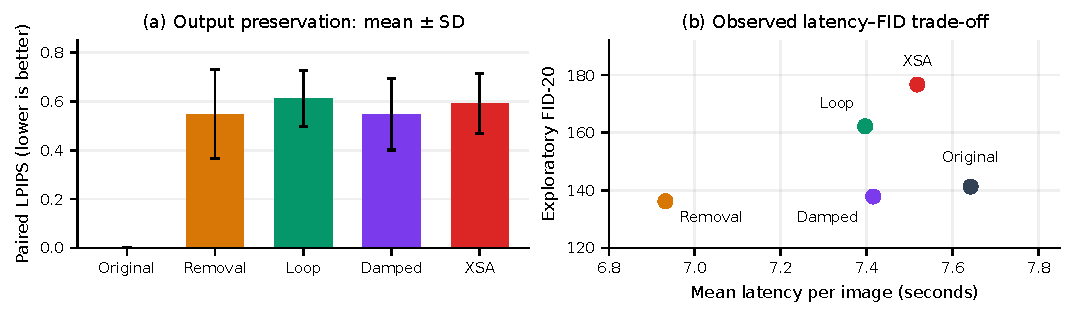
\includegraphics[width=\textwidth]{figures/milestone_summary.pdf}
 \caption{Observed trade-offs in the completed 20-image pilot. Left: mean paired
 LPIPS with sample SD. Right: latency versus exploratory FID; lower-left is
 desirable, but FID rankings are not reliable at this sample size. Damping
 labels refer to the fixed $0.5$ policy actually recorded in the manifests.}
 \Description{Two panels show paired output deviation and the latency--FID trade-off for the five methods. Damped and removed methods have similar mean LPIPS; all FID estimates are exploratory.}
 \label{fig:pilot}
\end{figure*}

\section{Next Experiments and Milestone Conclusion}
The code now supports 500 held-out images per class (5,000 per method), but
\textbf{those final results have not been generated}. At the observed rate,
five such runs require approximately 53 hours of sampling, plus evaluation.
We will freeze settings on validation, run the disjoint held-out seeds, and
check metric variability across additional seed sets rather than interpreting
small single-run FID changes. The key ablations are consecutive removed slots
and greater reuse counts (to separate fixed $0.5$ from harmonic $1/k$),
removal-budget and location sweeps, and XSA on/off under the same schedule.
Optional TPIPS aspects can supplement LPIPS if runtime permits; no aspect
scores or CLIP scores are currently claimed.

The milestone establishes a working frozen-weight comparison and exact
parameter savings. Preliminary output-preservation results favor controlled
residual updates over naive reuse, but a larger experiment is required to
determine whether either damping or XSA improves the quality--cost trade-off.

\paragraph{Code and attribution.}
The project notebook and tests are at
\href{https://github.com/cl-xy/cs5787-deep-learning/tree/81b8806}{\texttt{cl-xy/cs5787-deep-learning}, commit \texttt{81b8806}}.
We extend the official \href{https://github.com/facebookresearch/DiT/tree/ed81ce2229091fd4ecc9a223645f95cf379d582b}{DiT PyTorch sampling code}
with shared-block schedules, damping, XSA hooks, compact checkpoints,
class-matched references, provenance checks, and report exports. The code
supplement contains every notebook code cell and both test files; nine
regression tests, including 14 notebook checks, passed at this snapshot.
The optional appendix documents upstream code and libraries; no published
paper's reported numbers are presented as our measurements.

\bibliographystyle{ACM-Reference-Format}
\bibliography{references}
\ifdefined\IncludeCodeAppendix
 \clearpage\appendix% Optional supplement, excluded from the default 2--3-page milestone build.
\section{Code, Provenance, and Reproduction}
\label{app:code}
The accompanying snapshot contains all project notebook code cells and both
regression-test files as of commit \texttt{81b8806}. The output-free notebook
preserves the cell ordering and markdown instructions. The flat Python file
below is an archival listing, not a recommended batch entry point: run the
notebook interactively to control generation and optional evaluation.
The measured run predates harmonic damping; its executed-function snapshot
is preserved separately in \texttt{data/notebook\_sources.json}, and its
generation fingerprint begins \texttt{6da12ce572d7}.

\subsection{Code collected online and project changes}
\begin{itemize}
\item Official DiT source and demo: \url{https://github.com/facebookresearch/DiT},
including \texttt{run\_DiT.ipynb}, \texttt{models.py}, and the ancestral
diffusion implementation. The submodule is pinned to
\texttt{ed81ce2229091fd4ecc9a223645f95cf379d582b}; upstream code retains its
CC BY-NC 4.0 license. Its training code is not executed by this project.
\item The XSA mathematical operation is adapted from Looped-DiT:
\url{https://github.com/OpenSenseNova/Looped-DiT}. We implement the projection
through scoped hooks in the frozen DiT attention path rather than claiming
to reproduce that repository's trained model.
\item Training-free looping reference code:
\url{https://github.com/L-z-Chen/Training-Free-Looped-Transformer}.
Our progressive $1/k$ replacement schedule differs from its constant-$1/K$
integrator; no language-model evaluation results are reused here.
\item TeaCache source (related work, not executed):
\url{https://github.com/ali-vilab/TeaCache}.
\item Image sampling uses PyTorch, timm, and Diffusers:
\url{https://pytorch.org/}, \url{https://github.com/huggingface/pytorch-image-models},
and \url{https://github.com/huggingface/diffusers}.
The pretrained VAE is \url{https://huggingface.co/stabilityai/sd-vae-ft-mse}.
\item LPIPS and Clean-FID are used through their released libraries:
\url{https://github.com/richzhang/PerceptualSimilarity} and
\url{https://github.com/GaParmar/clean-fid}.
\item Optional TPIPS code is at
\url{https://github.com/adobe-research/TPIPS}; it is disabled in the measured run.
\item Imagenette data and metadata are from
\url{https://github.com/fastai/imagenette}. The full-resolution archive is
downloaded by torchvision; its original ImageNet class IDs are explicitly
mapped in the notebook.
\end{itemize}

The project-level changes include unique-module registration with explicit
execution schedules, block removal/reuse/damping, an inference-only XSA
adapter, compact checkpoint reconstruction, matched RNG streams,
CPU/MPS/CUDA support, calibration hooks, class-balanced reference preparation,
manifest validation, provenance fingerprints, bounded previews, and report
plots. They extend the sampling implementation within PyTorch; this is not
a TensorFlow-to-PyTorch conversion. \textbf{TODO before final submission:}
record each student's contributions and the exact source URL/credit for any
additional pasted team/Colab companion code not identifiable from the
repository. A code listing alone does not establish original authorship.

\subsection{Reproduction entry points}
Clone the project at the stated commit, initialize its DiT submodule, and run
\texttt{venv/bin/python -m pytest -q}. Use notebook sections 1--8 for the
validation pipeline and section 12 alone to regenerate figures from completed
saved artifacts. The larger held-out test in section 10 remains explicitly
disabled until validation choices are frozen. Do not rerun completed
generation folders or combine different source fingerprints in one comparison.

\onecolumn
\lstset{language=Python,basicstyle=\ttfamily\scriptsize,
 numbers=left,numberstyle=\tiny,numbersep=6pt,breaklines=true,
 breakatwhitespace=false,showstringspaces=false,columns=fullflexible,
 keepspaces=true,tabsize=4,frame=single,framerule=0.2pt,
 literate={—}{{---}}3 {–}{{--}}2 {−}{{-}}1 {→}{{$\to$}}1
 {↓}{{$\downarrow$}}1 {↑}{{$\uparrow$}}1 {α}{{$\alpha$}}1
 {×}{{$\times$}}1 {±}{{$\pm$}}1 {≤}{{$\leq$}}1 {≥}{{$\geq$}}1
 {…}{{...}}3 {’}{{'}}1}
\subsection{Complete notebook code cells}
\lstinputlisting{code/notebook_code.py}
\subsection{Notebook and damping regression tests}
\lstinputlisting{code/tests/test_notebook.py}
\subsection{Saved-report regression tests}
\lstinputlisting{code/tests/test_reports.py}

\fi
\end{document}
